\documentclass[11pt,letter,french]{article} 
\usepackage{babel}

%\usepackage[latin1]{inputenc}
\usepackage[parfill]{parskip} % Activate to begin paragraphs with an empty line rather than an indent
\usepackage{amsmath,amsthm,amssymb,bbm} %math stuff
\usepackage{placeins} % FloatBarrier
\usepackage{fancyhdr}
\usepackage{lastpage}
\usepackage{float}    % for fig.pos='H'
\usepackage{rotfloat} % for sidewaysfigure
%\usepackage{subfig}   % for subfigure
\usepackage{subcaption}  % an alternative package for sub figures
\usepackage{comment}
\usepackage[round]{natbib}   % omit 'round' option if you prefer square brackets
\bibliographystyle{plainnat}
\usepackage{setspace} %Spacing
\usepackage{graphicx,graphics}
\usepackage{booktabs,tabularx}
\usepackage{enumerate}
\usepackage{makecell}
\usepackage{xfrac}
\restylefloat{figure}
\usepackage{appendix}
\usepackage{color, colortbl, xcolor}
\usepackage{booktabs,dcolumn} % for use with texreg in R
\usepackage[pagebackref=true,bookmarks]{hyperref}
\hypersetup{
    unicode=false,          
    pdftoolbar=true,        
    pdfmenubar=true,        
    pdffitwindow=false,     % window fit to page when opened
    pdfstartview={FitH},    % fits the width of the page to the window
    pdftitle={004-Figures},    % title
    pdfauthor={SRB},     % author
    pdfsubject={Subject},   % subject of the document
    pdfcreator={SRB},   % creator of the document
    pdfproducer={SRB}, % producer of the document
    pdfkeywords={}, % list of keywords
    pdfnewwindow=true,      % links in new window
    colorlinks=true,       % false: boxed links; true: colored links
    linkcolor=black,          % color of internal links (change box color with linkbordercolor)
    citecolor=blue,        % color of links to bibliography
    filecolor=black,      % color of file links
    urlcolor=cyan           % color of external links
}
\usepackage{wrapfig}
\usepackage{todonotes}
\usepackage{ctable}


% my commands
\newcommand{\nd}{\noindent}
\newcommand{\ntodo}[2][]{\todo[#1]{\thesubsubsection{}. #2}}

% fancy header commands
\renewcommand{\headrulewidth}{0.3pt}
\renewcommand{\footrulewidth}{0.0pt}
\setlength{\textheight}{9.00in}
\setlength{\textwidth}{7.00in}
\setlength{\topmargin}{-1.1in}
\setlength{\evensidemargin}{-0.25in}
\setlength{\oddsidemargin}{-0.25in}
\renewcommand{\baselinestretch}{0.85}
\makeatletter
\makeatother
\lfoot{} \cfoot{ } \rfoot{{\small{\em Page \thepage \ of \pageref{LastPage}}}}

\usepackage{tcolorbox}
\usepackage{setspace}
\onehalfspacing


 \vspace{-8ex}
  \date{}
\usepackage{Sweave}
\begin{document}
\Sconcordance{concordance:report.tex:report.Rnw:%
1 192 1 51 0 4 1 4 0 7 1 4 0 7 1 4 0 259 1 4 0 5 1 4 0 5 1 4 0 6 1 4 0 %
22 1}

\pagestyle{plain}

\title{%
 Méthodes avancées en exploitation de donnée \\
  \large (MATH80619)}
\author{\begin{tabular}{ll}
    Estefan Apablaza-Arancibia & 11271806\\
        Adrien Hernandez & 11269225\\

    
\end{tabular}}
\maketitle

\section{Introduction}
In the first section of this paper, a literature review covers the neural networks and deep learners algorithms, focusing on different type of neural networks architecture; the purpose of adding multiple hidden layers and, ultimately, what are the challenges regarding the increase in computing time. Furthermore, in the methodology section, a list of deep learning projects are shown in order to understand some patterns and methods. Then, an exhaustive list of the R libraries allowing to build neural networks and deep learners models. Correspondingly, the advantages and disadvantages of each libraries, their capabilities as well as what you can expect when using them. To sum up, the last section will give concrete examples on how to implement the neural networks and deep learners models with these libraries, using real data.
\ntodo[inline]{Add more detail about deep learning integration}

\section{Litterature Review}
\subsection{What is Deep Learning and why use it?}
\begin{figure}[h]
    \centering
    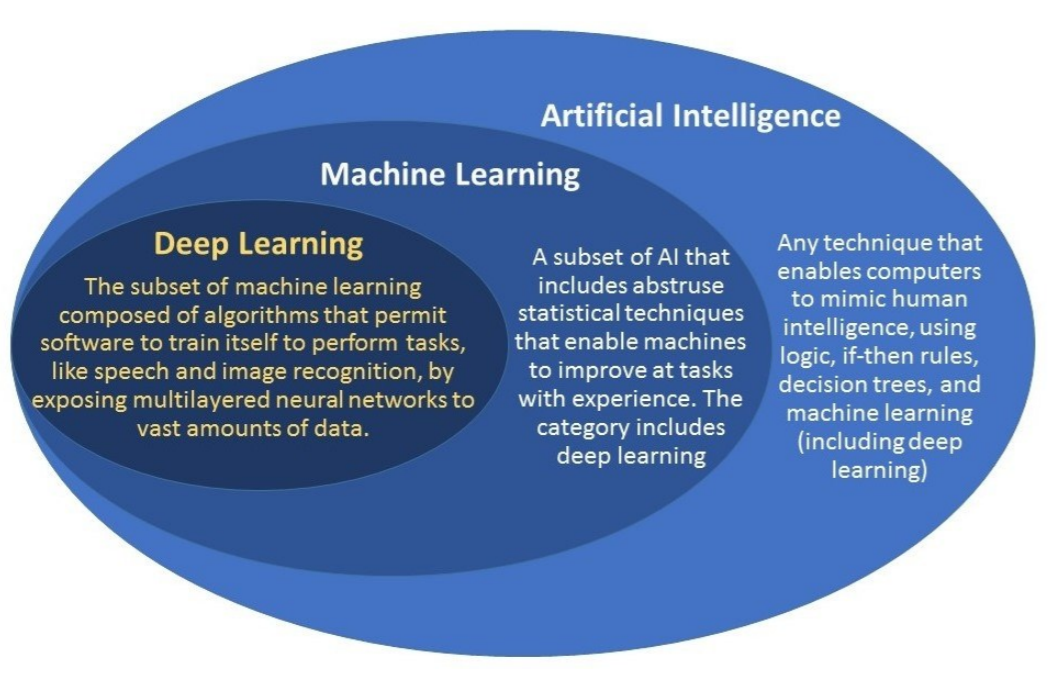
\includegraphics[width=0.4\textwidth]{deep learning.PNG}
     \caption{artificial intelligence vs machine learning vs deep learning}
     \label{fig:simule}
\end{figure}

Deep learning is a subset field of articial intelligence and can be seen as a specific way of doing machine learning. Deep learning algorithms can be seen as feature representation learning. Indeed, by applying to the data multiple non-linear transformations through the use of hidden layers, deep learning models have their own trainable feature extration capability making it possible to learn specific features from the data without needing a specific human domain expert. This means that deep learning models won't require the features extraction step that is essential for classic machine learning models. However, increasing the models capacity by adding hidden layers, requires increasingly computing power and slow down the training process of the model. The choice of hyperparameters, programming languages and memory management will therefore be important criteria to take into account will building deep learning models\\
Since the last decade, deep learning models have shown notable predictive power and have been revolutionizing an important number of domain such as computer vision, natural language understanding, fraud detection, health and much more.\\
We suggest reading this first chapter written by pioneers in the field: \url{https://www.deeplearningbook.org/contents/intro.html}
\ntodo[inline]{Très très intéressant:\url{https://r2018-rennes.sciencesconf.org/data/pages/Deep_with_R_1.pdf}}


\subsubsection{Feed Forward Neural Network}
\begin{wrapfigure}[11]{r}{0.4\textwidth}
  \begin{center}
    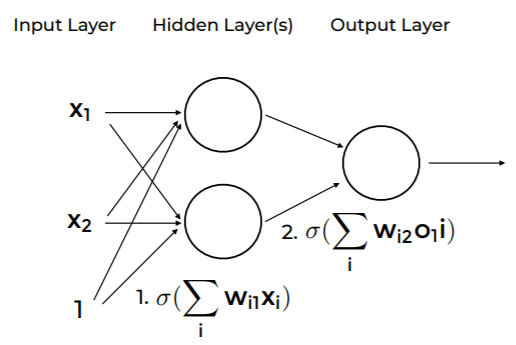
\includegraphics[width=0.4\textwidth]{feedforward_neural_networks.png}
  \end{center}
  \caption{feedforward neural networks}
  \label{fig:attention}
\end{wrapfigure}
"Deep feedforward networks, also called feedforward neural networks, or multilayer perceptrons(MLPs), are the quintessential deep learning models." (Bengio, Deep Learning)

Feedforward neural networks models are inspired from biology and by the way the human brain works. In a neural network, each neuron takes input from other neurons, processes the information and then transmits outputs to next neurons. Artificial neural networks follow the same process as each neuron will perform the weighted sum of inputs and will add a bias as a degree of freedom. It will then apply a non-linear transformation before outputting the information. \ntodo[inline]{ajouter formule mathematique du neurone}. Thus, the information goes forward in the network; neurons transmit information from the input layers towards the output layer. It is important to know that in a feedfoward neural networks the neurons of a same layer are not connected to each other; they do not allow any feedback connections within a same layer. If we want to allow this process, we will be looking at recurrent neural networks.\\
To get a detailed explanation of the theory of feedforward neural network we recommand to read this chapter: \url{https://www.deeplearningbook.org/contents/mlp.html}\\
To get a short but still useful summary we recommand this chapter: \url{https://www.dropbox.com/s/uh48e6wjs4w13t5/Chapter6.pdf?dl=0}

\subsubsection{RNN}
Recurrent neural networks are a type of neural networks architecture having proven state-of-art performance for solving tasks related to sequential data such as language traduction, generation or text classification. As a key differentiator from feedfoward neural networks, they include feedback loops connections and get an internal memory. One of their other advantage is to be able to handle input and ouput sequences that do not have the same length. TBC....
\\ To get a detailed explanation of the theory of recurrent neural networks we recommand to read this chapter: \url{https://www.deeplearningbook.org/contents/rnn.html}
\ntodo[inline]{expliquer les différent possibilité qu'il existe dans le monde deep learning (i.e. RNN, CNN , GNN , etc.). Si tu veux on peux expliquer les graphes aussi}
\subsubsection{CNN}
To get a detailed explanation of convolutional neural networks we recommand to read this chapter: \url{https://www.deeplearningbook.org/contents/convnets.html}

\ntodo[inline]{Recommend books for deep learning or maybe here the hype cyckle makes more sense}
\subsection{How to integrate Deep Learning in R}
Deep Learning with R \cite{deeplearningr}
\ntodo[inline]{Recommend books for deep learning that implements R}


\section{Methodology}
\ntodo[inline]{Give example of deep learning project pocedure}
\section{Available resources}
\ntodo[inline]{Très intéressant:\url{https://edu.kpfu.ru/pluginfile.php/419285/mod_resource/content/2/neural-networks-r.pdf}}
\ntodo[inline]{Faire une recherche exhaustive des ressources disponibles en R pour faire des analyses liées à ce sujet. Par exemple: fonctions R de base, packages sur les différentes plate-formes (CRAN, )}
According to the CRAN-R project website, we give a list of the different packages known in R allowing to use simple and deep neural network algorithms. \newline \url{https://cran.r-project.org/web/views/MachineLearning.html}
\subsection{Nnet}

\textbf{Nnet} (Ripley and Venables, 2016) allows to quickly train and fit a feed-forward neural networks with one hidden layer. This package does not allow to use more that one hidden layer, and does not have any feature to find the optimal number of neurones in the hidden layer. It is up to the analyst to build a loop to test by cross-validation, for exemple, the optimal hyperparameter values.\url{https://cran.r-project.org/web/packages/nnet/nnet.pdf}\\
\subsection{Popular packages}
\subsubsection{Keras}
\paragraph{Tensorflow}
\paragraph{CNTK}
\paragraph{Theano}

%$https://keras.rstudio.com/$
\subsubsection{Tensorlow}

\section{Packages not popular}

\paragraph{RSNNS}

Another package \textbf{RSNNS} (Bergmeir, 2019) allows to have access to a high view of the pakcage SNNS (Stuttgart Neural Network Simulator), containing several neural networks algorithms \ntodo[inline]{à creuser ce package}

\paragraph{Deepnet}

For deep learning algorithms, \textbf{Deepnet} (Rong, 2014), allows to us neural networks with several hidden layers. This package contains interesting features such as neural networks having their neurones' weight automatically initialized by a DBN (deep belief network) or a stacked autoencoder. (\ntodo[inline]{il fait aussi Boltzmann machine, à voir ce que c'est})\\

Another package, \textbf{RcppDL} (Kou and Sugomori, 2014), allows a simple use of deep neural netowkrsm including denoising autoencoders, stacked denoising autoencoder, restricted Boltzmann machines and deep belief nets.\\

\textbf{H2o} (LeDell, 2020) video qui explique h2o 
%$https://www.youtube.com/watch?v=g7drhm_SdbQ$
H2o is a "scalable open source machine learning platform that offers parallelized implementations of many supervised, unsupervised and fully automatic machine learning algorithms on clusters". This package allows to run H2o via its REST API through R and offers several advantages such as the ability ot know the computation time remaining when running a model.
Prerequisites to launch H2o, 64 bit Java 6+ if you want to open a h2o model that s more than 1 GB. 
R users: prerequisite R installed. Add R to your PATH. install.packages("h2o")
different syntax to work with h2o. read.csv = h2o.importFile. cbind = h2o.cbind. predict = h2o.predict. glm = h2o.glm, ...
According to KD Nuggets, "Recurrent Neural Networks and Convolutional Neural Networks can be constructed using H2o's deep water project throught others libraries such as Caffe and TensorFlow". "Some of the features of H2o deep learning models are: Automatic Adaptive learning rate, Model regularization, Model checkpointing, Grid Search". Source: 
%https://www.kdnuggets.com/2018/01/deep-learning-h2o-using-r.html



\textbf{Keras and tensorflow(backend)} (Falbel, 2019)\\

\textbf{CNTK-R (backend)}\\

\textbf{Theano (backend)}\\

%https://cran.rstudio.com/web/packages/keras/vignettes/backend.html$
\textbf{brnn}\\

\textbf{deepnlp}\\

\textbf{brnn}\\

\textbf{neuralnet} allows to plot the neural net (keras allows it too i think)\\

\ntodo[inline]{Ce mec parle de la gestion de la memoire en R avec keras, qui me semble utilise des numpy array en backend ... à creuser mais peut etre interessant d'en parler car le gros probleme de R pour le deep learning c'est sa gestion de la memoire $https://community.rstudio.com/t/deep-learning-in-r-memory-allocation/17541$}


\ntodo[inline]{Bonne ressource pour videos \url{https://www.youtube.com/user/westlandindia/videos}}
\begin{table}
\centering
\begin{tabular}{lllll}
Package      & Pro & Con & Actif & URL   \\
tensorflow R &     &     &       & Link  \\
Kera R       &     &     &       &       \\
MxNet        &     &     &       &      
\end{tabular}
\end{table}
\ntodo[inline]{Ici on pourrait faire un tableau avec tous les packages et donner les pour et les contres, ADRIEN: Le tableau je suis pas trop fan sachant qu on doit ecrire 20 pages sur ces librairies}
\section{Tutorials}
\ntodo[inline]{Encore à voir... on pourrait créer des tutoriels pour peut-être comparer}
\ntodo[inline]{Il faut trouver des datasets intéressantes à utiliser avec les differents packages}


\newpage

\bibliographystyle{IEEEtran} 

\bibliography{deep} % Entries are in the "refs.bib" file

\newpage
\begin{appendix}

\section{Code}
\textbf{Exemple de code utilisant h20 mais ce n' est pas du deep learning donc il faura l'adapter}

\ntodo[inline]{Le code doit aller ici ou faire un autre document. Il peut y avoir des bouts de code dans le texte si cela aide à la compréhension. Le code complet sera fourni à part dans un autre document (pas de limite de pages ici)}
\end{appendix}

\end{document}

